\chapter{Project Approach}
\setlength{\parindent}{15pt}
\label{ch:proj_appr}

\section{Design Process}
\label{sec:desi_proc}
%Entire design process, from baseline to final, including iteration process

In the baseline report \cite{baseline} concepts were generated that could deal with the problem on hand. In the midterm report \cite{midterm} a trade-off was performed to see which concept would be the best to do so. Now that a concept is chosen, further detailed design can be done to ensure the requirements can be met. The first step taken into the detailed design was finding out which sub-systems there are. Once the sub-systems


coming up with departments which would work on various aspects of the aircraft. In total, five departments were created, which would cover all the aspects. The departments are listed in \autoref{tab:departments}.

\begin{table}[]
    \centering
    \begin{tabular}{c|c}
    Dep     &  \\
         & 
    \end{tabular}
    \caption{Caption}
    \label{tab:my_label}
\end{table}

The first step taken into the detailed design was coming up with tools to help aid the design process. One of the major tools that aided the design process was the $N^2$ chart which shows the interrelations between sub-systems, shown in \autoref{sec:subs_inte}.

\section{Verification \& Validation Procedure}
\label{sec:veri_vali_proc}

In this section, the verification and validation procedures are analysed and explained. First, in \autoref{sec:verification}, the verification method used for each requirement is illustrated. Then, in \autoref{sec:validation}, validation procedures for different tools, models and the final product are discussed. The actual execution of the verification and validation is not discussed in this section but is documented throughout the report since it is also executed continuously throughout the design phase.

\subsection{Verification}%of requirements
\label{sec:verification}

In order to verify requirements, different methods can be used such as inspecting, analysing, demonstrating or testing. Verifying by inspection means using human senses to verify the requirement. Verification by analysis means verifying by mathematical theorems that the product satisfies the requirement. Verification by demonstration means verifying by operating the UAV under specific conditions to verify that the results are as expected. Verification by tests can be done by checking the compliance of the product with the requirement under representative circumstances. The difference between test and demonstration is that testing requires a more specialised test setup and equipment. \autoref{tab:verification} gives an overview of all of the requirements and the method that can be used to verify them. In this table abbreviations are used: A = analysis, D = demonstration, I = inspection and T = test. 

\begin{table}[htb]
\centering
\caption{Requirements Verification Methods}
\label{tab:verification}
\begin{tabular}{ll|ll|ll}
\toprule
\textbf{Requirement} & \textbf{Method} & \textbf{Requirement} & \textbf{Method} & \textbf{Requirement} & \textbf{Method}\\ \midrule
SYS-C-1                 &A                       &SYS-OP-2.7              &D &SYS-C-2                 &A \\\hdashline                      
SYS-OP-2.8.2            &D &SYS-S-2                 &A                       &SYS-OP-2.8.6            &D \\\hdashline
SYS-L-2                 &T                       &SYS-OP-2.8.7            &I    &SYS-L-3                 &T, A, D and I  \\\hdashline            
SYS-OP-2.8.8            &D  &SYS-R-1                 &I                       &SYS-OP-2.9.2            &D \\\hdashline
SYS-ENV-1.4             &T                       &SYS-OP-2.9.3            &D &SYS-ENV-1.5             &A   \\\hdashline                    
SYS-OP-2.9.4            &D &SYS-ENV-1.6             &D                       &SYS-PF-1.1              &A      \\\hdashline
SYS-ENV-2.1             &D                       &SYS-PF-1.2              &T         & SYS-ENV-2.2             &D       \\\hdashline                
SYS-PF-1.3              &T          &SYS-ENV-2.5             &I                       &SYS-PF-1.4              &T          \\\hdashline
SYS-PH-1.1              &I                       &SYS-PF-2.1              &D &SYS-PH-1.2              &I     \\\hdashline                  
SYS-PF-2.2              &D &SYS-PH-2                &D                       &SYS-PF-2.3              &D \\\hdashline
SYS-PH-4.3              &T                       &SYS-PF-2.4              &T          &SYS-PH-4.4              &T       \\\hdashline                
SYS-PF-3                &A      &SYS-OP-1.1              &D                       &SYS-PF-4                &A      \\\hdashline
SYS-OP-1.5              &I                       &SYS-VS-1.1              &D &SYS-OP-1.7              &D       \\\hdashline                
SYS-VS-1.2.1            &T                          &SYS-OP-2.1              &A                       &SYS-VS-1.2.2            &T          \\\hdashline
SYS-OP-2.2              &A                       &SYS-VS-1.2.3            &D &SYS-OP-2.3              &I  \\\hdashline     
SYS-VS-1.2.4            &D                       &SYS-OP-2.4              &D                       &SYS-VS-2.1              &T          \\\hdashline
SYS-OP-2.5.3            &T                       &SYS-VS-2.2              &T          &SYS-OP-2.5.4            &T         \\\hdashline              
SYS-VS-2.3              &T          &SYS-OP-2.5.5            &T                       &SYS-VS-3                &I    \\\hdashline
SYS-OP-2.9.5 & T &&&&    \\
\bottomrule
\end{tabular}
\end{table}

During the DSE it is not possible to verify the requirements by test, demonstration or inspection Therefore, only the requirements that can be verified by analysis are analysed and verified in \autoref{ch:desi_spec}.

\subsection{Validation}
\label{sec:validation}

In this section, the validation methods for the requirements, the tools and models used and the final product are presented.

Prove that all of the requirements are VALID (Verifiable, Achievable, Logical, Integral and  Definitive), has already been performed during their generation. 

Different tools will be used in order to create a model of a system. These include commonly used tools such as for example CATIA, EXCEL, and PYTHON but also less common tools can be used such as XFLR5. The calculation methods of the well known programs are validated by experience since they have been continuously validated by experts in various fields within industries. The less common tools need to be validated by analysis in order to check if they are the correct tools to use for a certain purpose. The inputs given by the user will be validated using inspection, meaning reviewing all the inputs and checking the formulas for typos.

%experience ---> different input where we know the outputs already (use of same model)
%comparison ---> use different models or test data to calculated same outputs using same inputs

The model validation will check if the models used to analyse systems and products are the correct models and if they reflect the physical phenomenon as accurately as required. Models can be validated in three different ways: by experience, by analysis and by comparison. Validating a model by experience is checking if the model produces the expected outcome while using various inputs. Validating by analysis means showing that the elements of the model are correct and are correctly integrated. Comparison validation compares the outcome of the model with independent models of proven validity or actual test data. The model validation procedures differ from model to model. The execution of the model validation will be documented in \Cref{ADD CORRECT REFERENCES}. 

Validation of the product is answering the question if the product accomplishes the intended purpose. In other words, does the product fulfil the Mission Need Statement (MNS). Qualification tests and acceptance tests need to be performed for the system product validation. A stress test and simulations can be used as qualification. Mission scenario tests and operations readiness tests are possible acceptance tests that can be used. Since these tests can only be performed when at least a prototype of the system exits, product validation by analysis needs to take place in this stage of the design. When the product fulfils all the requirements, the product also fulfils the MNS. Hence, the product can be validated by checking if all the requirements are verified. This is documented in \autoref{sec:comp_matr}.
\nomenclature{MNS}{Mission Need Statement}

\section{Sustainable Development Strategy}
\label{sec:sust_deve_stra}

Life Cycle Assessment (LCA) is chosen to analyse and develop sustainability into the design process and the product. Based on a LCA guide \cite{lca}, a structure of LCA can be represented by \autoref{fig:lcatriangle}. Goal and scope needs to defined as a first step of LCA in order to proceed inventory analysis, impact assessment and improvement assessment. \autoref{fig:lcawheel} shows 6 phases of a product and sustainability of the hybrid UAV will be assessed for each phase.
\nomenclature{LCA}{Life Cycle Assessment}

\begin{figure}[H]
    \centering
    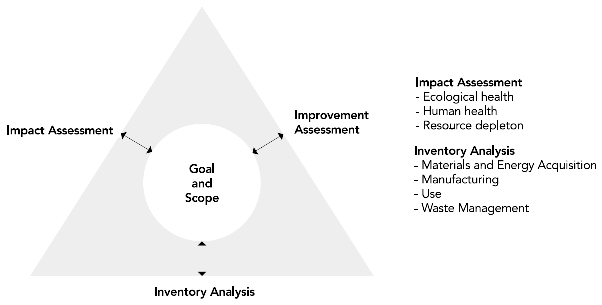
\includegraphics[width=0.8\textwidth]{ProjectApproach/Figures/LCAtriangle.pdf}
    \caption{Technical Framework for Life Cycle Assessment}
    \label{fig:lcatriangle}
\end{figure}

\begin{figure}[H]
    \centering
    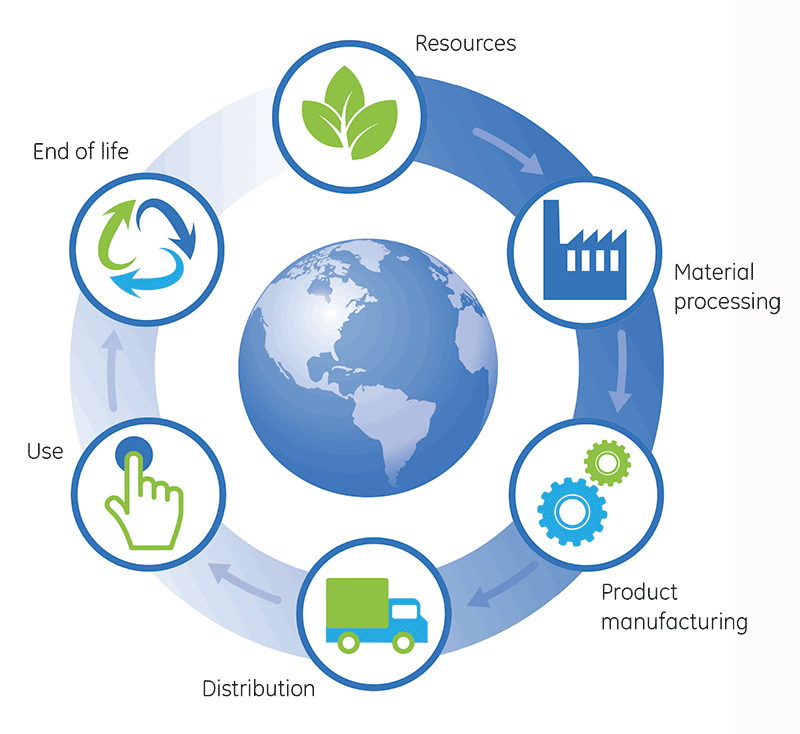
\includegraphics[width=0.6\textwidth]{ProjectApproach/Figures/lcadiagram.jpg}
    \caption{Life Cycle Assessment Wheel}
    \label{fig:lcawheel}
\end{figure}

The technical framework and the actual LCA for ????? (WILL BE REPLACED WITH A NAME) will be elaborated in \autoref{ch:life_cycl_asse}.


